% https://tex.stackexchange.com/q/224408/
\documentclass[12pt]{article}
\usepackage[a4paper,margin=3cm]{geometry}
%\usepackage[papersize={6.67in,3.75in},margin=1.5cm]{geometry}
\usepackage[brazil]{babel}
\usepackage[utf8]{inputenc}
\usepackage[T1]{fontenc}
\usepackage{amsmath}
\usepackage{enumitem}
\usepackage{graphicx}
\usepackage{xsim}
\usepackage{setspace}
\usepackage{xcolor}

\newcommand{\content}{Termometria}
\usepackage{fancyhdr}

\newcommand{\aspas}[1]{``#1''}

\lhead{\content}
\cfoot{}
\rfoot{\thepage}

\author{J. R. Oliveira}
\date{\today}
\title{\content}

\DeclareExerciseTranslation{Brazil}{exercise}{Exercício}
\DeclareExerciseTranslation{Brazil}{solution}{Solução}

\DeclareExerciseTagging{difficulty}
\DeclareExerciseTagging{type}
\DeclareExerciseTagging{typequestion}
\DeclareExerciseTagging{author}

\usepackage{needspace}

\DeclareExerciseProperty{shortsolution}

% we'll use a description list for the shortsolutions:
\newcommand\printshortsolutions{%
    \ForEachUsedExerciseByType{%
      \def\ExerciseType{##1}%
      \def\ExerciseID{##2}%
      \GetExercisePropertyT{shortsolution}
        {%
          \par\noindent\textbf{##3}.
           ####1%
        }%
    }%  
}

\usepackage{environ,etoolbox}
\NewEnviron{shortsolution}{\SetExpandedExerciseProperty{shortsolution}{\expandonce{\BODY}}}

\newcommand*\includeQuestion[1]{%
\XSIMexpandcode{\printexercise{exercise}{\GetExerciseIdForProperty{ID}{#1}}}%
}

\newcommand*\includeSolution[1]{%
\XSIMexpandcode{\printsolution{exercise}{\GetExerciseIdForProperty{ID}{#1}}}%
}

\DeclareExerciseEnvironmentTemplate{simpleExercise}
  {\par\noindent\textbf{\GetExerciseProperty{counter}}.~}
  {\par\smallskip}
  
\DeclareExerciseEnvironmentTemplate{simpleSolution}
{\par\noindent\textbf{\GetExerciseName~\GetExerciseProperty{counter}}:\newline}
{\par\smallskip}

\xsimsetup{exercise/template=simpleExercise,
           solution/template=simpleSolution
}
\DeclareExerciseCollection{termER}
\DeclareExerciseCollection{termEasyER}
\DeclareExerciseCollection{col:cap1Term}

% comment/uncomment to print solutions
%\renewcommand*\includeSolution[1]{}

\begin{document}

\onehalfspacing

\maketitle
\newpage
\tableofcontents
\newpage

%\pagestyle{fancy}


%\section*{Questões}
%\includeQuestion{Q001}
%\includeQuestion{Q002}
%\includeQuestion{Q003}

%\section*{Soluções}
%\includeSolution{Q001}
%\includeSolution{Q002}
%\includeSolution{Q003}

%\section{Exercícios Aleatórios}
\section{Temperatura e Calor}
\begin{itemize}
    \item Temperatura:
    \begin{itemize}
            \item Macroscópico: quantidade que informa quão quente ou frio está um objeto em relação a algum padrão;
            \item Microscópico: grau de agitação térmica de moléculas.
    \end{itemize}
    \item Instrumento de medida: termômetro (analógico, digital, infravermelho...);
    \item Sensação térmica: sensação de \aspas{mais quente} ou \aspas{mais frio};
    \item Calor: energia transferida de uma coisa a outra por causa da diferença de temperatura;
    \item Equilíbrio térmico: estado em que os corpos apresentam a mesma temperatura; 
    \item Lei de Zero da Termodinâmica: \aspas{Se dois corpos A e B estão separadamente em equilíbrio térmico com um terceiro corpo C, então A e B estão em equilíbrio térmico entre si}. (Se $T_{a}=T_{c}$ e $T_{b}=T_{c}$, então $T_{a}=T_{b}$). 
\end{itemize}

\section{Escalas Termométricas}

\begin{itemize}
    \item Celsius: escala usada no Brasil e na maior parte dos países (conhecida como escala centígrada);
    \item Fahrenheit: escalas mais utilizadas em países de língua inglesa;
    \item Kelvin: escala mais utilizada meios científicos;
    \item Relação entre as principais escalas: \[\dfrac{T_{C}}{5}=\dfrac{T_{F}-32}{9}=\dfrac{T_{K}-273}{5}\]
    De forma mais simplificada:
        \begin{equation}\label{eq:tctf}
            \dfrac{T_{C}}{5}=\dfrac{T_{F}-32}{9}
        \end{equation}
        \begin{equation}\label{eq:tftk}
            \dfrac{T_{F}-32}{9}=\dfrac{T_{K}-273}{5}
        \end{equation}
            \begin{equation}\label{eq:tctk}
            T_{C}=T_{K}-273
        \end{equation}
        \item Variações: $\Delta T_{F}= 1,8\cdot\Delta T_{C}=1,8\cdot\Delta T_{K}$;
    \item Escalas Arbitrárias: utiliza-se proporção simples.
\end{itemize}

\section{Exercícios Resolvidos}
\collectexercises{termER}
\xsimsetup{type=ER}
\begin{exercise}[ID=Q201001, difficulty=easy, type=ER, typequestion=open]
    Maria usou um livro de receitas para fazer um bolo de fubá. Mas, ao fazer a tradução do livro do inglês para o português, a temperatura permaneceu em Fahrenheit ($^\circ F$). A receita disse que o bolo deve ser levado ao forno a $392\;^\circ F$ e permanecer nessa temperatura por 30 minutos. Qual é a temperatura em graus Celsius que Maria deve deixar o forno para não errar a receita?
\end{exercise}
\begin{shortsolution}
	$200\;^\circ C$.
\end{shortsolution}
\begin{solution}
	Dado que $T_{F}=392\;^\circ F$ e utilizando a equação de conversão entre Celsius e Fahrenheit, temos: \[\dfrac{T_{C}}{5}=\dfrac{392-32}{9}\] Desta forma, isolando $T_{C}$, obtemos: \boxed{T_{C}=200\;^\circ C}
\end{solution}

\begin{exercise}[ID=Q201002, difficulty=easy, type=ER, typequestion=open]
    Determine o valor da temperatura de zero absoluto nas escalas Celsius e Fahrenheit.
\end{exercise}
\begin{shortsolution}
	$-273\;^\circ C$ e $-459,4\;^\circ F$.
\end{shortsolution}
\begin{solution}
	A temperatura de zero absoluto é igual a $0\;K$.\\Utilizando a equação de conversão entre Celsius e Kelvin, temos: \[T_{C}=0-273\] Logo, isolando $T_{C}$, obtemos: $T_{C}=-273\;^\circ C$.\\ Agora, utilizando a equação de conversão entre Fahrenheit e Kelvin, temos: \[\dfrac{T_{F}-32}{9}=\dfrac{0-273}{5}\] Logo, isolando $T_{F}$, temos: $T_{F}=-459,4\;^\circ F$.\\ Assim, podemos concluir que: \boxed{0K=-273\;^\circ C=-459,4\;^\circ F}    
\end{solution}

\begin{exercise}[ID=Q201003, difficulty=easy, type=ER, typequestion=open]
    Determine a única temperatura cuja indicação é a mesma nas escalas Celsius e Fahrenheit.
\end{exercise}
\begin{shortsolution}
$-40\;^\circ$
\end{shortsolution}
\begin{solution}
	A condição é $T_{C}=T_{F}=T$. Portanto, substituindo na equação de conversão entre Celsius e Fahrenheit, temos o seguinte: \[\dfrac{T}{5}=\dfrac{T-32}{9}\] Assim, isolando $T$, obtemos: \boxed{T=-40\;^\circ}\\
	Logo, $-40\;^\circ C$ é igual a $-40\;^\circ F$.    
\end{solution}

\begin{exercise}[ID=Q201004, difficulty=easy, type=ER, typequestion=open]
    O verão de 1994 foi particularmente quente nos Estados Unidos da América. A diferença entre a máxima temperatura do verão e a mínima no inverno anterior foi de $60\;^\circ C$. Qual o valor dessa diferença na escala Fahrenheit?
\end{exercise}
\begin{shortsolution}
	$108\;^\circ F$
\end{shortsolution}
\begin{solution}
	A relação entre a variação de temperatura na escala Fahrenheit e a escala Celsius é a seguinte: $\Delta 1\;^\circ C=\Delta 1,8\;^\circ F$.\\ Desta forma, a partir de uma proporção simples, obtemos: \[\dfrac{x}{1,8}=\dfrac{60}{1}\] Logo, \boxed{x=108\;^\circ F}\\ Ou seja, uma variação de $60\;^\circ C$ equivale a uma variação de $108\;^\circ F$.   
\end{solution}

\begin{exercise}[ID=Q201005, difficulty=easy, type=ER, typequestion=open]
    O cientista francês René Réaumur criou uma escala muito usada no passado, que adotava os seguintes valores: $0\;^\circ R$ para o ponto de gelo e $80\;^\circ R$ para o ponto vapor, ambos sob pressão normal. Calcule a temperatura nessa escala correspondente a $35\;^\circ C$.
\end{exercise}
\begin{shortsolution}
	$28\;^\circ R$
\end{shortsolution}
\begin{solution}
	Utilizando proporção entre as escalas, obtemos o seguinte: 
	\[\dfrac{35-0}{100-0}=\dfrac{T_{R}-0}{80-0}\]
	Assim, após isolarmos $T_{R}$, encontramos que: \boxed{T_{R}=28\;^\circ R}\\ Ou seja, $35\;^\circ C=28\;^\circ R$.    
\end{solution}

\begin{exercise}[ID=Q201006, difficulty=medium, type=ER, typequestion=open]
    Um estudante de física criou uma escala ($^\circ X$), comparada com a escala Celsius ele obteve o seguinte gráfico:
    \begin{figure}[ht] 
        \centering
        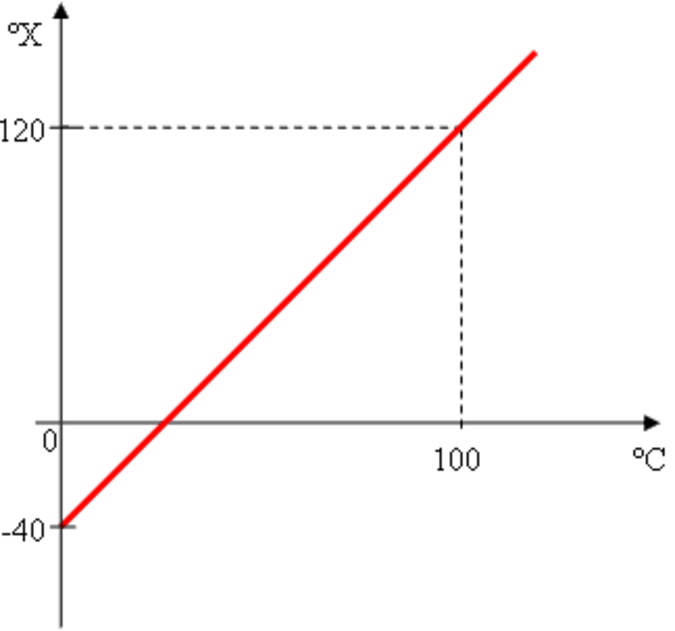
\includegraphics[scale=0.3]{graph1.pdf}
        %\caption{Exercício}
        \label{fig:graphterm1}
    \end{figure}
    \begin{enumerate}[label=\alph*),nosep]
        \item Qual a equação de conversão entre a escala $X$ e a escala Celsius?
        \item Qual a temperatura do corpo humano ($37\;^\circ C$) nesta escala?
    \end{enumerate}
\end{exercise}
\begin{shortsolution}
	$19,2\;^\circ X$
\end{shortsolution}
\begin{solution}
	\noindent
\begin{enumerate}[label=\alph*),nosep]
	\item A partir do gráfico, é possível escolher dois pontos $P_{1}=(-40,0)$ e $P_{2}=(100,120)$. Fazendo uma proporção entre as escalas, obtemos:
	\[\dfrac{T_{X}-(-40)}{120-(-40)} = \dfrac{T_{C}-0}{100-0}\]
	Desta forma:
	\[\boxed{T_{X}=\dfrac{8 \cdot T_{C}}{5} - 40}\]
	\item Substituindo $37\;^\circ C$ na relação anterior, encontramos: \boxed{19,2\;^\circ X}
\end{enumerate}   
\end{solution}
\collectexercisesstop{termER}
\includeQuestion{Q201001}
\includeSolution{Q201001}
\includeQuestion{Q201002}
\includeSolution{Q201002}
\includeQuestion{Q201003}
\includeSolution{Q201003}
\includeQuestion{Q201004}
\includeSolution{Q201004}
\includeQuestion{Q201005}
\includeSolution{Q201005}
\includeQuestion{Q201006}
\includeSolution{Q201006}
\section{Exercícios Propostos}

\section{Gabaritos}

\printshortsolutions

\section{Soluções}
\printsolutions*[headings=false,collection=termER]



%\collectexercises{col:cap1Term}
%\input{bqCap1TermStu.tex}
%\collectexercisesstop{col:cap1Term}

\end{document}

%\section{Problemas}
% set hint through option:

%\section{Gabaritos}
%\printgabs

%\section{Soluções}
%\printsolutions[headings=false]

%\end{document}
